\chapter{Estado del arte} \label{ich:estado_arte}

Procedemos a realizar un estudio del estado del arte para el problema que buscamos resolver. Consultaremos los mejores trabajos para la tarea de \textit{retrieval} en reconocimiento facial invariante a la edad sobre el conjunto de datos \textit{FG-Net}.

Posteriormente en \sectionref{isec:base_datos_usada} estudiaremos las bases de datos disponibles para resolver un porblema de \textit{AIFR}. En base a este estudio posterior y motivados por el trabajo de \cite{informatica:best_fgnet_model}, \textbf{nuestro enfoque va a ser el siguiente}: realizar un entrenamiento sobre el conjunto de datos \textit{CACD}, y usar \textit{FG-Net} para validar nuestro modelo.

En este sentido, no es de interés estudiar los resultados de modelos sobre \textit{CACD}, porque estamos usando dicho conjunto para entrenar, no para evaluar el rendimiento del modelo. Además, la mayoría de trabajos que estudiaremos más adelante siguen nuestro enfoque, usando un \textit{dataset} de tamaño considerable para entrenar y evaluando sobre \textit{FG-Net}. Es decir, su \textit{dataset} de entrenamiento no tiene por qué ser \textit{CACD}. Con esto queda claro que lo que realmente nos interesa son los resultados sobre \textit{FG-Net}.

\section{Interés del área de estudio} \label{isec:interesareaestudio}

Empecemos viendo el interés de este área de estudio. Para ello podemos realizar una búsqueda en \textit{SCOPUS}, buscando trabajos sobre \textit{AIFR}, filtrando el área de estudio al de las ciencias de la computación. Para realizar dicha búsqueda usamos las siguientes palabras clave o \textit{keywords}:

\begin{lstlisting}[caption=\textit{Keywords usadas para la búsqueda en \textit{SCOPUS}. Búsqueda realizada el 17 de Septiembre de 2023}, label=code:scopus_search, captionpos=b]
    TITLE-ABS-KEY ( age  AND invariant  AND face  AND recognition )  AND  ( LIMIT-TO ( SUBJAREA ,  "COMP" ) )
\end{lstlisting}

Con dichas \textit{keywords} obtenemos la siguiente gráfica:

\begin{figure}[H]
    \centering
    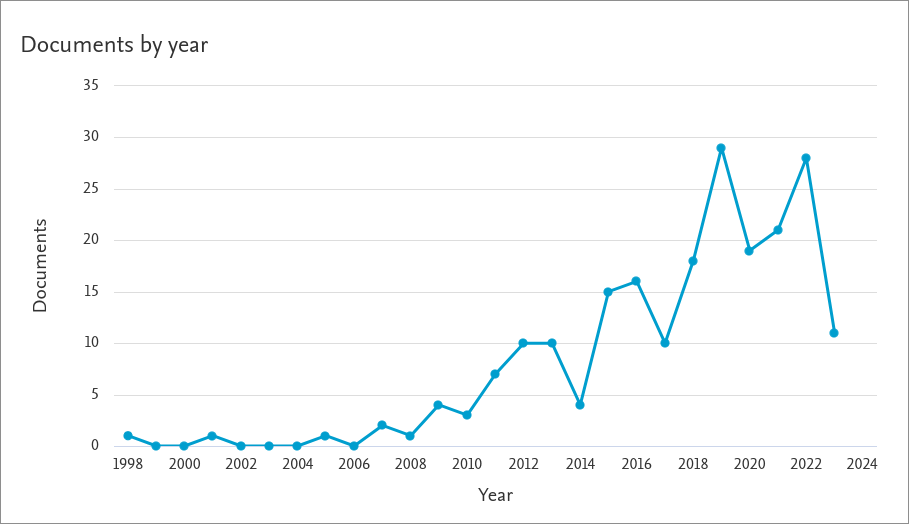
\includegraphics[width=0.7\textwidth]{informatica/scopus_search_histogram}
    \caption{Resultados de la búsqueda en \textit{SCOPUS} usando las \textit{keywords} del \coderef{code:scopus_search}}
\end{figure}

Vemos que, a partir de 2012 este área de estudio gana bastante popularidad. Coincide este momento con la aparición de \textit{AlexNet}, que da paso a la popularidad de las redes convolucionales profundas en el campo de la visión por computador. Sin tener en cuenta el último año (pues, en el momento de la consulta, sigue en curso y está lejos de acabar), no vemos que la tendencia siga al alza, pudiendo llegar a pensar que la popularidad de este campo se está estancando. Aunque habría que tener en cuenta condiciones externas, como la pandemia de \textit{COVID}, que podrían explicar la bajada notable en los años 2020 y 2021.

Veamos también la popularidad de la técnica \textit{triplet loss}, pues estamos proponiendo algunas variaciones sobre esta técnica. Las \textit{keywords} usadas fueron:

\begin{lstlisting}[caption=\textit{Keywords usadas para la búsqueda en \textit{SCOPUS} para consultar la popularidad del \textit{triplet loss}. Búsqueda realizada el 17 de Septiembre de 2023}, label=code:scopus_search_tripletloss, captionpos=b]
    TITLE-ABS-KEY ( triplet  AND loss )
    AND  ( LIMIT-TO ( SUBJAREA ,  "COMP" ) )
\end{lstlisting}

La búsqueda con estas \textit{keywords} produce la siguiente gráfica:

\begin{figure}[H]
    \centering
    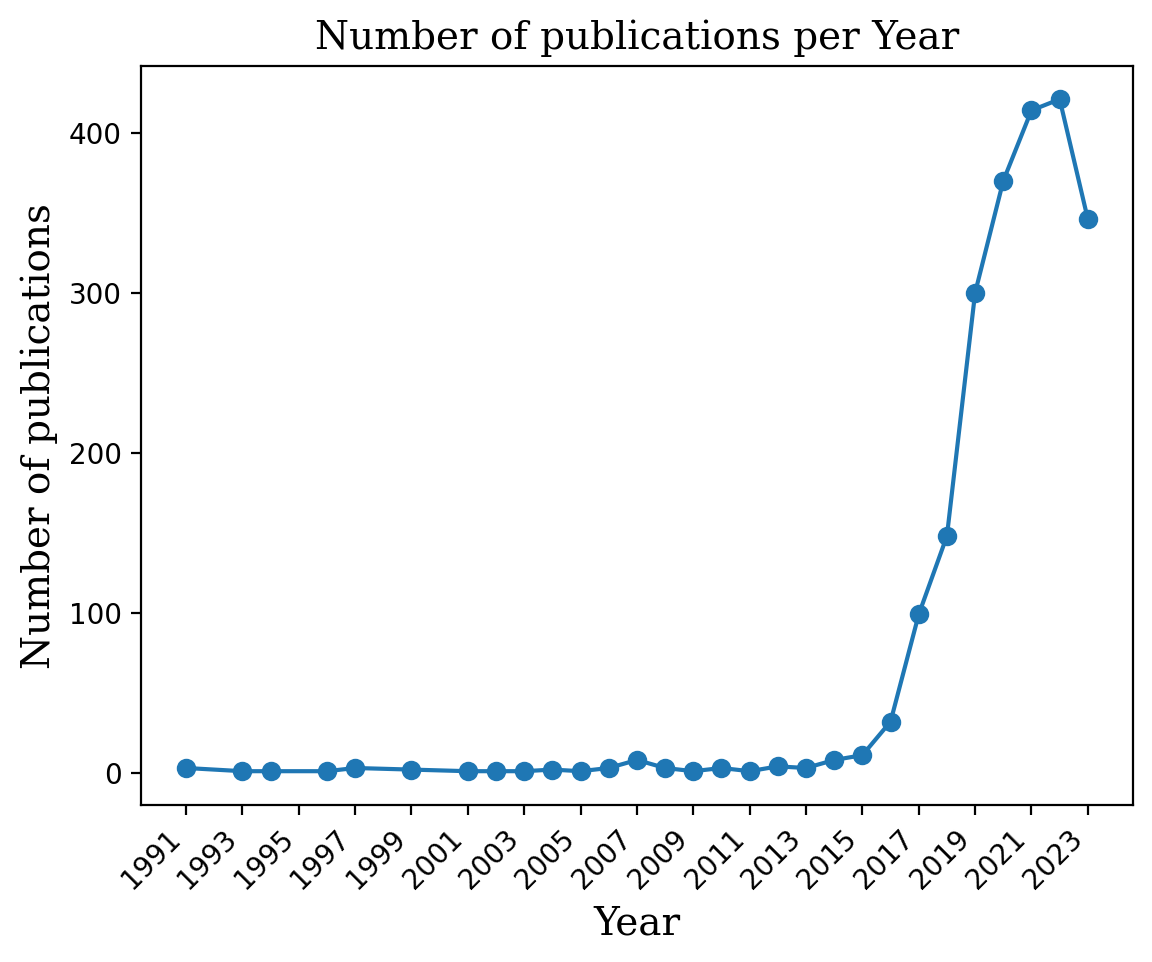
\includegraphics[width=0.7\textwidth]{informatica/scopus_search_tripletloss}
    \caption{Resultados de la búsqueda en \textit{SCOPUS} usando las \textit{keywords} del \coderef{code:scopus_search_tripletloss}. El descenso en el número de publicaciones en el último año puede ser debido a que no hemos finalizado el año o a que tenemos una tendencia a la baja}
\end{figure}

Vemos que entre 2017 y 2018 esta técnica da un grandísimo salto en popularidad. Sin embargo, en el último año la popularidad ha caído drásticamente. Aunque todavía no haya pasado el tiempo suficiente para observar el progreso de la tendencia, la caída en el último año es tan grande que pensamos que dicha tendencia va a seguir a la baja.

Por otro lado, estamos usando nuevas técnicas para computar \textit{triplet loss}. Dichas técnicas fueron introducidas en \cite{informatica:principal}. \textbf{En dicho trabajo se intenta resolver una tarea de re-identificación, que difiere de nuestra tarea de \textit{retrieval} para reconocimiento facial invariante a la edad}. Por lo tanto, buscamos trabajos que hayan aplicado \textit{triplet loss} en el campo del \textit{AIFR}. Aplicamos la siguiente búsqueda:

\begin{lstlisting}[caption=Keywords usandos para la búsqueda de trabajos que combinen \textit{AIFR} y \textit{triplet loss} en \textit{SCOPUS}, label=code:scopus_search_especifico, captionpos=b]
    TITLE-ABS-KEY ( age AND invariant AND face AND recognition, AND triplet AND loss )  AND  ( LIMIT-TO ( SUBJAREA ,  "COMP" ) )
\end{lstlisting}

La búsqueda determinada por \coderef{code:scopus_search_especifico} no produce ningún resultado. \textbf{SCOPUS no tiene constancia de ningún trabajo que aplique \textit{triplet loss} al campo del \textit{AIFR}}. Y esto, sin considerar que nuestro trabajo introduce nuevas técnicas que mejoran el uso del \textit{triplet loss} clásico, desarrollado en \sectionref{isec:triplet_loss}.

Así que, cuando veamos en \sectionref{ich:conclusiones} que no obtenemos buenos resultados, tendremos que \textbf{justificar el por qué basándonos únicamente en el trabajo presente}, puesto que \textbf{ningún trabajo ha intentado resolver una tarea de \textit{AIFR} usando \textit{triplet loss}}.

\section{Mejores modelos de \textit{retrieval} para el \textit{dataset} \textit{FG-Net}}

En esta sección vamos a introducir qué técnicas y tendencias han sido las que mayor éxito han tenido en el ámbito del \textit{AIFR} trabajando sobre el \textit{dataset} de \textit{FG-Net}. Realizaremos algunos apuntes sobre los trabajos que mejores modelos han producido, pero nos centraremos en las tendencias generales.
Como ya hemos visto en \sectionref{isec:interesareaestudio}, ninguno de estos trabajos usará \textit{triplet loss}. Por lo tanto, será complicado justificar las diferencias entre nuestros resultados y los del estado del arte.

Este estudio se fundamenta en los tres mejores trabajos hasta la fecha, en cuanto a que obtienen los mejores resultados sobre \textit{FG-Net}:

\begin{itemize}
    \item \entrecomillado{When Age-Invariant Face Recognition Meets Face Age Synthesis: A Multi-Task Learning Framework} \cite{informatica:best_fgnet_model} que propone el modelo \textit{MTLFace}. Dicho modelo se construye en dos pasos, que consisten en:
        \begin{enumerate}
            \item Aprender dos \textit{features} incorreladas: edad e identidad. Para ello se usa una arquitectura basa en modelos de atención
            \item A partir de esto, se optimiza una función multiobjetivo, para resolver dos tareas:
                    \begin{itemize}
                        \item Estimar la edad de una persona a partir de una imagen suya
                        \item Reconocimiento facial, es decir, determinar si en dos imágenes aparece o no la misma persona
                    \end{itemize}
            En dicho proceso se usa una red generativa adversaria, o \textit{GAN}.
        \end{enumerate}
    \item \entrecomillado{Decorrelated Adversarial Learning for Age-Invariant Face Recognition} \cite{informatica:dal} que propone el algoritmo de aprendizaje \textit{DAL}. En la misma línea que el trabajo anterior, se aprenden dos características incorreladas, una para la edad y otra para la identidad. Optimizamos la incorrelación entre edad e identidad a partir de un enfoque adversario
    \item \entrecomillado{Look Across Elapse: Disentangled Representation Learning and Photorealistic Cross-Age Face Synthesis for Age-Invariant Face Recognition} \cite{informatica:aim} que propone el modelo \textit{Age Invariant Model} o \textit{AIM}. De nuevo, se extraen dos características incorreladas a partir de un enfoque adversario. Del modelo \textit{GAN} se consigue extraer un generador de imágenes hiperrealista
\end{itemize}

En estos tres trabajos, podemos ver los siguientes puntos en común:

\begin{itemize}
    \item Los tres trabajos buscan aprender dos \textit{features} incorreladas. Una \textit{feature} se corresponderá a la identidad asociada a la imagen, y la otra se corresponderá a la edad de la persona que aparece en la imagen
    \item Los tres trabajos usan redes generativas adversarias, conocidas comúnmente como \textit{GANs}, con el mismo objetivo. Dada una edad objetivo y una imagen de ejemplo de un individuo, generar una imagen del mismo individuo con la edad objetivo. Como siempre, la tarea del discriminador es diferenciar entre imágenes reales e imágenes sintéticas creadas por la componente generativa
    \item Todos los trabajos proponen la creación de un nuevo \textit{dataset} de grandes dimensiones sobre el que realizar el entrenamiento. Esto deja claro que \textit{FG-Net} no es suficiente para entrenar un modelo lo suficientemente potente. Lo que \textbf{justifica nuestro enfoque de usar otro \textit{dataset}} mucho más grande para entrenar y emplear \textit{FG-Net} exclusivamente para validar el modelo obtenido
\end{itemize}

Estas similitudes tan grandes marcan una fuerte tendencia de trabajo en este área de estudio. Algunas diferencias entre los trabajos son:

\begin{itemize}
    \item El discriminador de \textit{DAL} busca maximizar la correlación entre las dos \textit{features} de las que hemos hablado
    \item El generador de \textit{AIM} es el de mejor calidad, llegando a ser fotorealista
    \item \textit{MTLFace} usa, en vez de redes convolucionales clásicas, mecanismos basados en atención
\end{itemize}

Veamos ahora el modelo generativo obtenido en \textit{MTLFace}:

\begin{figure}[H]
    \centering
    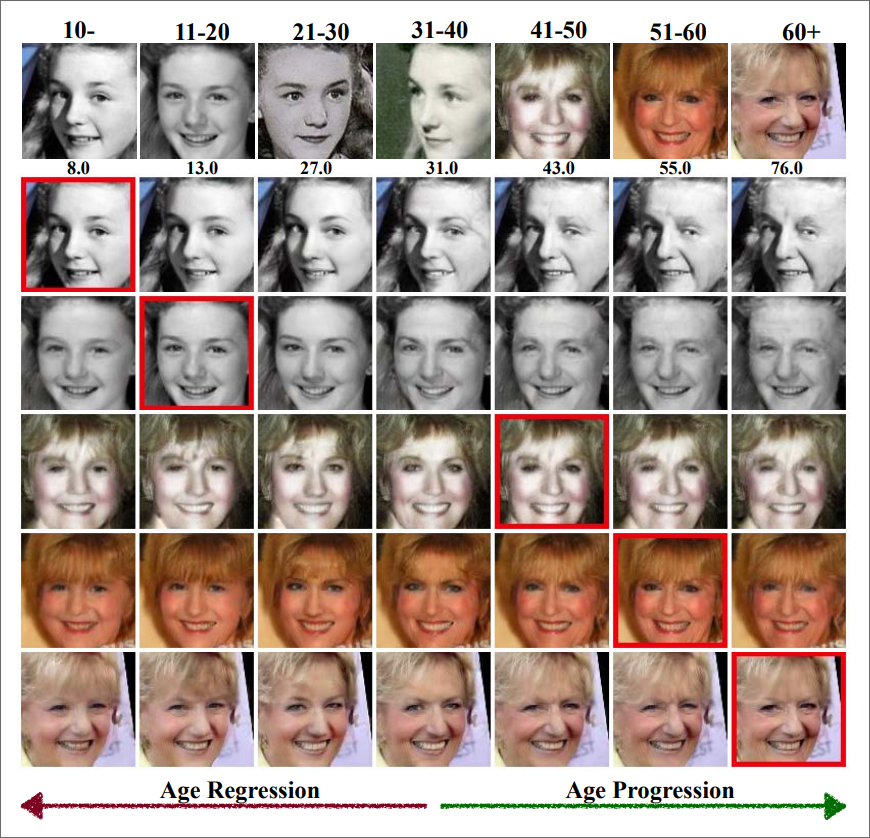
\includegraphics[width=0.6\textwidth]{informatica/mtlface_generativo}
    \caption{Ejemplo de los resultados del modelo generativo usado en el entrenamiento de \textit{MTLFace}. La primera fila muestra imágenes reales de una persona en distintas etapas de su vida. Las siguientes filas son imágenes generadas cuando se da como entrada la imagen marcada en rojo. Imagen extraída de \cite{informatica:best_fgnet_model}}
\end{figure}

Este generador no es tan bueno como el de \textit{AIM}, que llega a ser fotorealista, como muestra la siguiente imagen:

\begin{figure}[H]
    \centering
    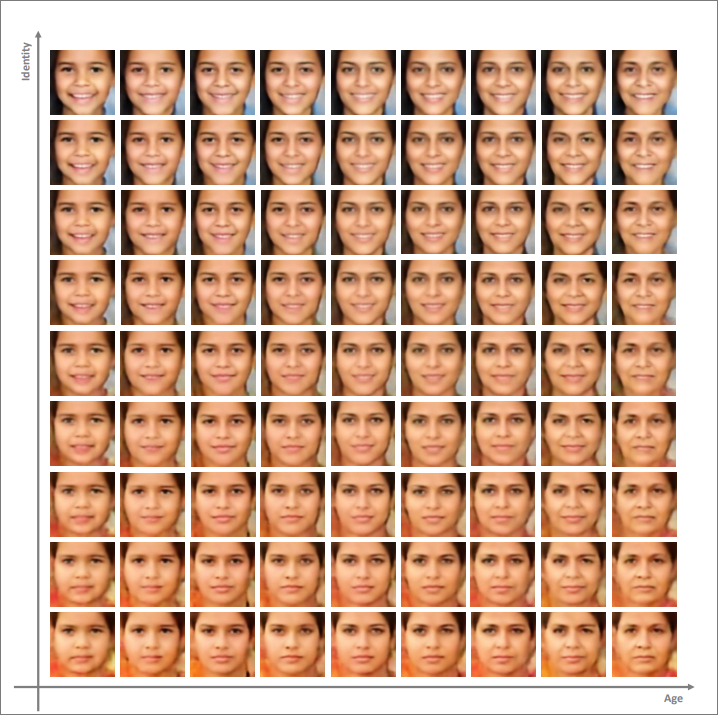
\includegraphics[width=0.6\textwidth]{informatica/aim_manifold}
    \caption{Espacio aprendido por \textit{AIM}, continuo sobre las \textit{features} de edad (eje horizontal) e identidad (eje vertical). El fotorealismo es evidente. Imagen extraída de \cite{informatica:aim}}
\end{figure}

La siguiente imagen muestra cómo \textit{DAL} busca aprender dos \textit{features} incorreladas:

\begin{figure}[H]
    \centering
    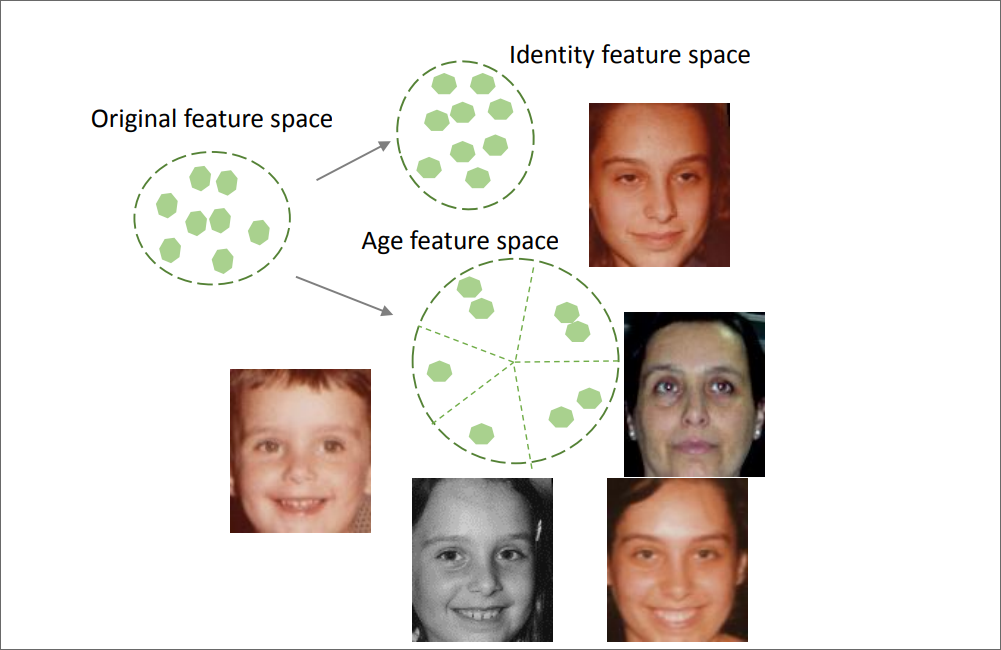
\includegraphics[width=0.6\textwidth]{informatica/dal_descomposicion}
    \caption{Ejemplo de cómo \textit{DAL} descompone la información en dos \textit{features}: una de edad y otra de identidad. Estas imágenes muestran como, fijada la componente de identidad, podemos variar la componente de edad. Imagen extraída de \cite{informatica:dal}}
\end{figure}

Mostramos ahora, de forma resumida, una comparativa de los resultados obtenidos por los trabajos que acabamos de estudiar. Usamos la métrica \textit{Rank@1} \footnotemark para comparar estos resultados:
\footnotetext{Si el lector no está familiarizado con la métrica \textit{Rank@k}, en \sectionref{isubs:rank_at_k} definimos qué es esta métrica}

\begin{table}[H]
\centering
\begin{tabular}{|l|l|l|l|l|}
    \hline
    Modelo & Dos \textit{features} incorreladas & Uso de \textit{GAN} & Modelo subyacente & \textit{Rank@1} \\
    \hline

    \textbf{\textit{MTLFace}} & Sí & Sí & Modelo basado en atención & \textbf{94.78} \\
    \textit{DAL} & Sí & Sí & \textit{CNN} & 94.5 \\
    \textit{AIM} & Sí & Sí & \textit{CNN} & 93.20 \\
    \hline

\end{tabular}
\caption{Resultados \textit{Rank@1} de los principales modelos estudiados del estado del arte sobre el \textit{dataset} \textit{FG-Net}}
\end{table}

Y ahora, usando la comparativa que aparece en \cite{informatica:best_fgnet_model}, mostramos los resultados de otros modelos, cuyos trabajos no hemos estudiado en detalle:

\begin{table}[H]
\centering
\begin{tabular}{|l|l|}
    \hline
    Modelo & \textit{Rank@1} \\
    \hline
    HFA & 69.00 \\
    MEFA & 76.20 \\
    CAN & 86.50 \\
    LF-CNN & 88.10 \\
    AIM & 93.20 \\
    DAL & 94.50 \\
    \textbf{MTLFace} & \textbf{94.78} \\
    \hline
\end{tabular}
\caption{Resultados \textit{Rank@1} de algunos modelos sobre el \textit{dataset} \textit{FG-Net}. Datos extraídos de \cite{informatica:best_fgnet_model}}
\end{table}

En base a todo esto extraemos las siguientes \textbf{conclusiones}:

\begin{itemize}
    \item \textbf{No existen trabajos previos que empleen \textit{triplet loss} para resolver una tarea de \textit{AIFR}}. Por lo tanto, no podremos contrastar los resultados obtenidos con modelos que operen de una forma parecida
    \item \textbf{Los mejores modelos sobre \textit{FG-Net} emplean técnicas mucho más avanzadas} que las presentadas en este trabajo. El aprendizaje de dos \textbf{\textit{features} incorreladas}, una para la edad y otra para la identidad, en base a \textbf{redes generativas adversarias}, es el punto común principal
    \item Por lo tanto, \textbf{parece que nuestra propuesta no va a ser lo suficientemente potente} como para obtener los resultados aquí mostrados. Para afirmar esto deberíamos realizar un estudio experimental en profundidad, que queda fuera del alcance de este trabajo. A pesar de esta sospecha, sería realmente interesante lograr resultados ligeramente competentes, pues obtendríamos un modelo mucho más ligero a partir de un entrenamiento mucho más fácil de realizar, tanto por los recursos como por las técnicas empleadas
\end{itemize}
